\pdfoutput=1
\documentclass[pra,twocolumn,showpacs,amsmath,amssymb]{revtex4-2}

\usepackage{graphicx}%Include figure files
\usepackage{dcolumn}%Align table columns on decimal point
\usepackage{bm}% bold math
\usepackage[section]{placeins} %force no floats before section
\usepackage{float}

\setlength{\parskip}{1em}

%\nofiles

\begin{document}

\title{Project 5: Quantum Tunneling of Wave Packets in One Dimension}


\author{Christopher McGlinn}
\affiliation{Department of Physics and Astronomy, University
of Delaware, Newark, DE 19716-2570, USA}

\begin{abstract}
In this experiment we explore the effect of quantum tunneling on a wave packet. For this we will use a matrix algorithm to compute the position over time of the wave packet, and introduce a potential barrier. We will show that the potential barrier causes a reflection and transmission wave, something that is not possible in classical mechanics, but is possible in quantum mechanics.
\end{abstract}

\pacs{03.65.Xp}


\maketitle

\section{Introduction} \label{sec:intro}

Quantum tunneling was first discovered as an offshoot of radioactivity by Henri Becquerel in 1896. The process occurs when a wave encounters a potential barrier. In classical mechanics, the wave would reflect off the barrier and travel in the opposite direction. However, in quantum mechanics, a portion of the wave transmits through the barrier and another portion reflects off of it. This relation is dictated by the time dependent Schrodinger equation:
\begin{eqnarray}
i\hbar \frac{\partial \psi}{\partial t} = - \frac{\hbar^2}{2m} \frac{\partial^2 \psi}{\partial x^2} + V(x)\psi
\end{eqnarray}
\par This relationship describes the motion of a wave in the space-time domain. This equation can be simplified for one-dimensional motion to the following:
\begin{eqnarray}
\frac{\partial \psi}{\partial t} = \frac{i\hbar}{2m} \frac{\partial^2 \psi}{\partial x^2}
\end{eqnarray}
\par In the experiment, we will introduce a potential barrier in the path of this wave. What we will see is that when the wave encounters, depending on the thickness of the barrier, the wave will both reflect and transmit about the barrier.
\par Furthermore, we will see that this relationship can be simplified into a "plane wave". This simplification will give us certain quantities, ideally the reflection and transmission coefficients.
\par These quantities will be calculated using the Crank-Nicholson method. This will give us a matrix we can use to use to solve the system as it evolves over time.

\section{Method} \label{sec:method}

First we must normalize the Schrodinger equation. This will allow us to effectively treat $\hbar$ and m as equal to 1. We can simplify the equation to the following relationship:
\begin{align}
\psi(x,t=0) = \frac{1}{2\pi \sigma^2}^{1/4} e^{\frac{-(x-x_o)^2}{4\sigma^2}} e^{ik_o (x-x_o)}
\end{align}
Here, $\sigma^2$ corresponds to the width of the wave. This and $k$ have the following relationships:
\begin{align}
    \sigma^2 &= \left\langle x^2 \right\rangle - \left\langle x \right\rangle^2 \\
    k &= \sqrt{\frac{2mE}{\hbar^2}}
\end{align}
Here $\left\langle x^2 \right\rangle$ corresponds to the expectation value of the wave. We can then calculate the numeric value for $\sigma$ and see if it corresponds our initial conditions. We can also calculate the total probability of the system $P$. This can be done using the following equations:
\begin{align}
    P = \int dx \psi^* \psi \\
    \left\langle x \right\rangle = \int dx \psi^* x \psi\\
    \left\langle x^2 \right\rangle = \int dx \psi^* x^2 \psi
\end{align}
This will verify that our solution in (3) is correct. 
\par After this we can find the transmissions and reflections coefficients using the following set of equations:
\begin{align}
    T = &\frac{1}{1 + \frac{V_O^2 \sinh^2(\frac{L}{\hbar}\sqrt{2m(V_o - E)}}{4E(V_o - E)}} \\
    R &= 1 - T
\end{align}
If we look at the transmission and reflection as functions of an incident wave $\psi = A e^{ikx}$, we can then use these values to verify our analytical approach.

\begin{figure}[t!]
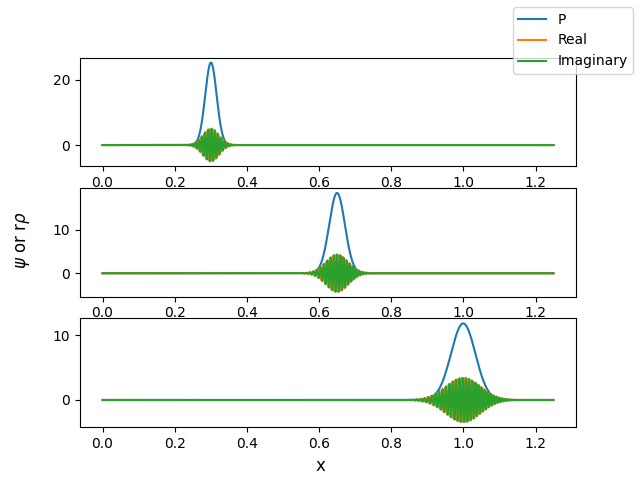
\includegraphics[scale=0.5]{psi_x_wo.png}
\caption{Propagation of wave packet through time for $\sigma^2 = 2.5 \times 10^{-4}$}\label{Poincare0.5}
\end{figure}

\par These will be calculated using the following matrix:
\[
  A =
  \left[ {\begin{array}{ccccccc}
    Q_1 & -iq & 0 & \cdots & \cdots & 0 & 0\\
    -iq & Q_2 & -iq & 0 & \ddots & \vdots & 0\\
    0 & -iq & Q_3 & \ddots & \ddots & \vdots & \vdots\\ 
    \vdots & 0 & \ddots & \ddots & \ddots & 0 & \vdots \\
    \vdots & \ddots & \ddots & \ddots & Q_{n-2} & -iq & 0\\
    0 & \cdots & \cdots & 0 & -iq & Q_{n-1} & -iq\\
    0 & 0 & \cdots & \cdots & 0 & -iq & Q_n\\
  \end{array} } \right]
\]
Where $Q = 1 + 2iq + \frac{i\delta t}{2} V_l$. This also gives us a B matrix where the $-iq$ are $iq$ and $Q = 1 - 2iq -\frac{i\delta t}{2}V_l$. Once we have these matrices, we can relate them together to give us the following equation:
\begin{align}
    \psi^{n+1} = A^{-1} B \psi^n
\end{align}
This relationship will allow us to follow the wave through time. Unless otherwise stated, the initial conditions are as follows:
\begin{align}
    x_o &= 0.3 & k_o &= 700 \notag\\
    \sigma^2 &= 2.5 \times 10^-4 & \Delta t &= 5 \times 10^-7 \notag \\
    \Delta t &= 5 \times 10^-7 \notag
\end{align}

\section{Results} \label{sec:results}

To begin, let us look at the motion of a wave packet through time without a potential barrier. In figure 1 we see the motion of our initial wave over time. The wave moves through space as expected. $\sigma^2$ increases with time as the probability expands. This is something that can be calculated through equation 4. We can find that, analytically, $\left\langle x \right\rangle = 0.30034$, $\left\langle x^2 \right\rangle = 0.090455$, and thus $\sigma^2 = 0.00025$. We can also verify that the probability remains within a reasonable difference from 1 using equation 6, which is calculated to within $10^{-15}$, which is reasonably close to 1. This validates that our method confirms our solution in equation 3.
\par Now let us look at the same wave packet, but with a larger width. In figure 2, $\sigma^2$ is increase by one order of magnitude. As you can see, the wave propagates much like it does in figure 1. However, $sigma^2$ increase faster than it did. This is confirmed by looking at the expectation value. The peak of the probability decreases at a much faster rate, thus giving more of an emphasis to the $\left\langle x^2 \right\rangle$ in equation 4.
\par Using our analytical solution in equation 9, we can calculate the transmission coefficient as a function of barrier width. In figure 3, we see that if the barrier width is too large, the wave will not transmit through the barrier, that is, $T = 0$. This also shows that if the barrier is sufficiently small we will get a much greater value for $T$. This will mean that more of the wave will transmit through the barrier.
\par For reference, figure 4 shows the potential barriers used in the following analysis. The width will be adjusted as needed.
\par Now let us see what happens when we introduce a potential barrier at $x = 0.6$. In figure 5, we see the propagation of the wave in this scenario. As you can see, the barrier causes the wave to both reflect and transmit through. We can also see the wave hit the barrier and the reflected wave interacts with the incident wave. However, the wave moves as expected from the given equations.

\begin{figure}[t!]
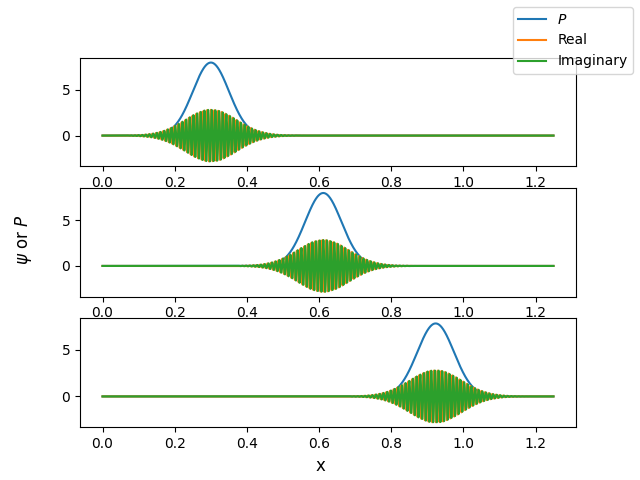
\includegraphics[scale=0.5]{psi2_x_wo.png}
\caption{Propagation of wave packet through time for $\sigma^2 = 2.5 \times 10^{-3}$}\label{Poincare0.5}
\end{figure}

\begin{figure}[t!]
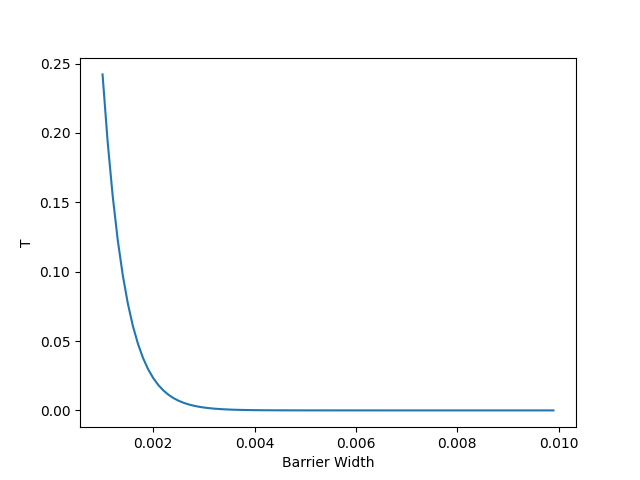
\includegraphics[scale=0.50]{t_d.png}
\caption{Transmission coefficient as a function of barrier width}\label{Poincare1}
\end{figure}

\begin{figure}[t!]
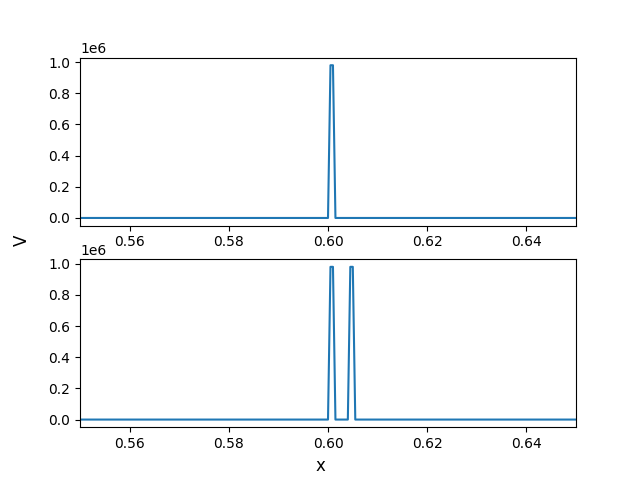
\includegraphics[scale=0.5]{V_x.png}
\caption{Propagation of wave packet through time for $\sigma^2 = 2.5 \times 10^{-3}$}\label{Poincare0.5}
\end{figure}

\begin{figure}[t!]
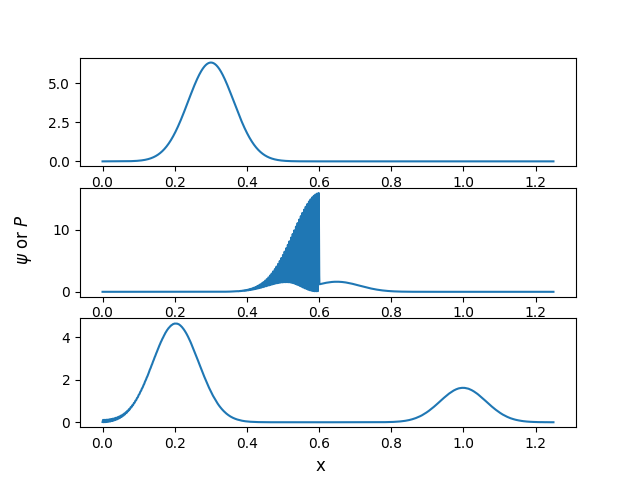
\includegraphics[scale=0.50]{Barrier01.png}
\caption{Propagation of wave packet through time with a potential barrier of width $L = 0.001$}\label{Poincare9}
\end{figure}

\par This phase transition, while continuous, is only first order. However, since the temperature is below the critical temperature of the system, spin flipping is much less likely to occur.
\par This is further explained when looking at a system that is where flipping is more likely to occur. In figure 3, the transition of the magnetization from -1 to 1 is a more smooth transition. The figure displays a second order transition. Since there is more energy in the system, spin flipping is more likely to occur. This allows for them to occur at values closer to 0, ever when the field is opposing the spin.

\begin{figure}[t!]
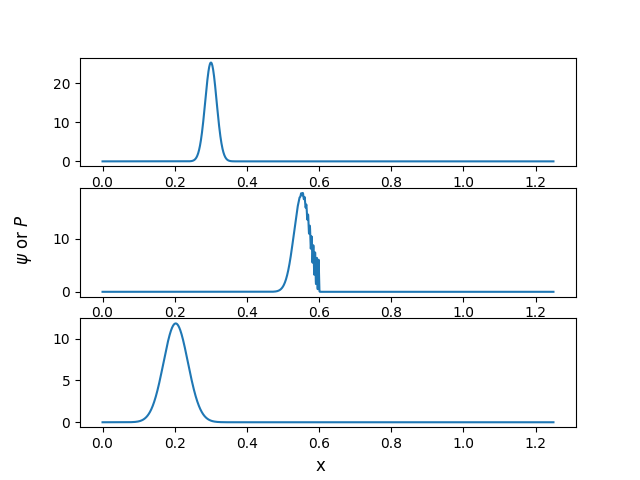
\includegraphics[scale=0.50]{Barrier05.png}
\caption{Propagation of wave packet through time with a potential barrier of width $L = 0.005$}\label{autocorr}
\end{figure}

\par If we increase the width of the barrier, we see that less of the wave is transmitted. In figure 6, we increased the barrier width to $L = 0.005$. This caused the wave to hit the barrier and seemingly fully reflect off of it. Again, we see the reflection interact with the incident wave at the time of impact.
\par Furthermore, if we increase the width yet again, we expect that the wave will continue to fully reflect off of the barrier. In figure 7, the barrier width was increased to $L=0.01$. As expected, we see the wave interact with the barrier in the same way that it did in figure 6.

\begin{figure}[t!]
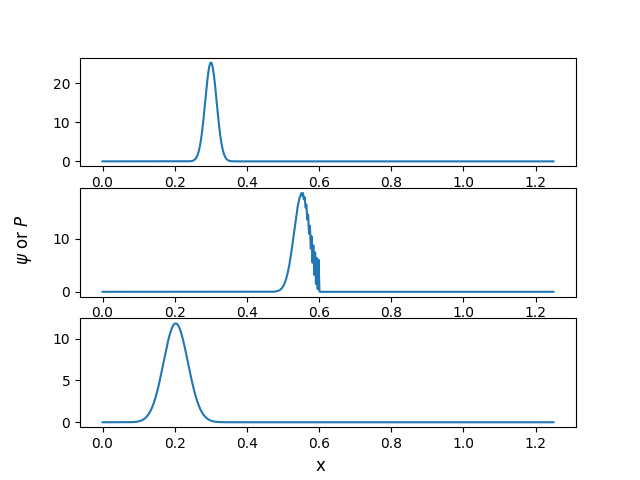
\includegraphics[scale=0.50]{Barrier1.png}
\caption{Propagation of wave packet through time with a potential barrier of width $L = 0.01$}\label{autocorr}
\end{figure}

\par Finally, we can explore the impact of a second barrier located at a distance 0.004 between the interiors. In figure 8, we see this interaction. The barrier causes the wave to reflect and transmit in the space between until it is fully transmitted through either of the barriers. You can see this by looking at the peak in the probability in that region. This also shows at final time when, unlike the single barrier, the transmission rate is greater than the reflection rate.
\par We can also explore the impact that a change in initial conditions may have. In figure 9, we decreased $k_o$ to a value of 620. As you can see, this caused resonance in the wave. Thus a small change in initial conditions can have a big impact on how the wave interacts with the barriers.

\begin{figure}[t!]
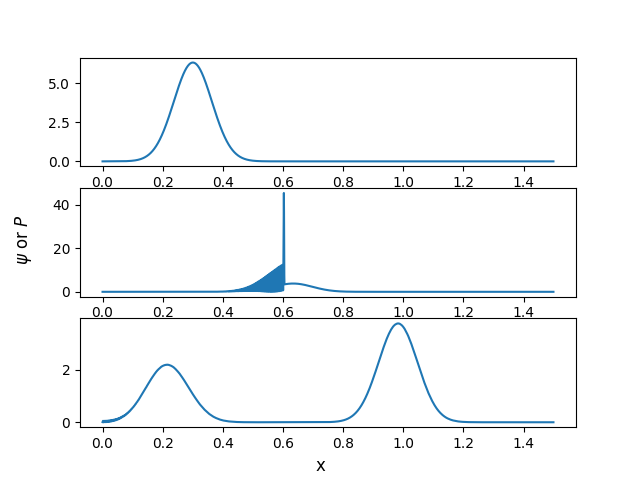
\includegraphics[scale=0.50]{2Barrier.png}
\caption{Propagation of the wave packet through a two potential barrier system}\label{Poincare0.5}
\end{figure}

\begin{figure}[t!]
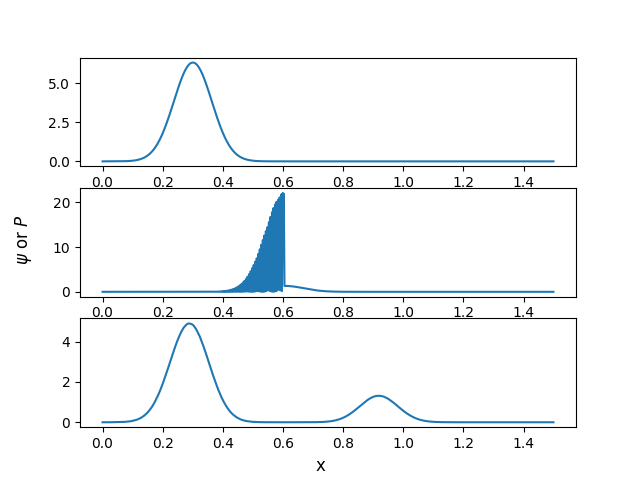
\includegraphics[scale=0.50]{2Barrier2.png}
\caption{Propagation of the wave packet through a two potential barrier system with $k_o = 620$}\label{Poincare0.5}
\end{figure}

\begin{figure}[t!]
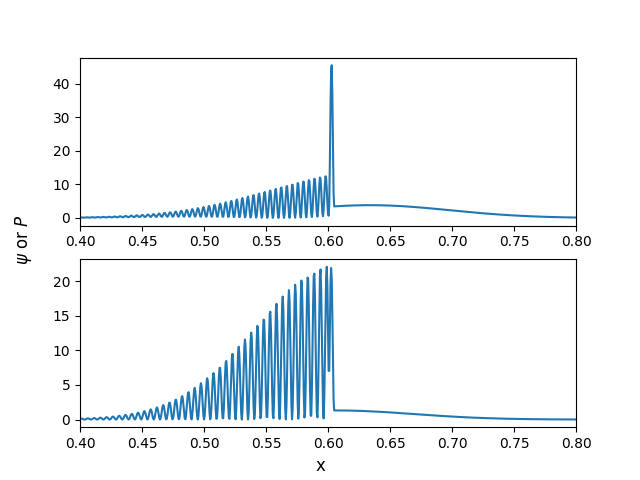
\includegraphics[scale=0.50]{close_up.png}
\caption{Close up look at the point of impact for both two potential barrier systems}\label{autocorr}
\end{figure}

\par To get a better picture of this interaction, we can look at a close up of the time of impact for both of the system. In figure 10, we see this time.We the peak caused by the two barriers in the first case as well as the resonance caused by the change of initial conditions in the second case.

\section{Conclusion} \label{sec:conclusion}

In conclusion, we were able to successfully show how a wave propagates through space-time. We saw the wave move when there were no potential barriers to interact with. We also saw the wave move in the presence of potential barriers. Changes to the initial conditions made impacts on these interactions. An increase in barrier width caused more of the wave to be reflected and changes in the initial conditions caused resonance in the two barrier system. These interesting results are of much discussion. These results would not be possible in a purely classical mechanics world. However, as we know, this does correspond to real-world events.

\begin{thebibliography}{9}
\bibitem{}Nicholas J. Giordano and Hisao Nakanish, \emph{Computational Physics}, (Pearson Prentice Hall, Upper Saddle River NJ,2006).
\end{thebibliography}

\end{document}